\documentclass[../main]{subfiles}
\begin{document}

\Large
\begin{tabu}{clr}
	\multirow{6}{1in}{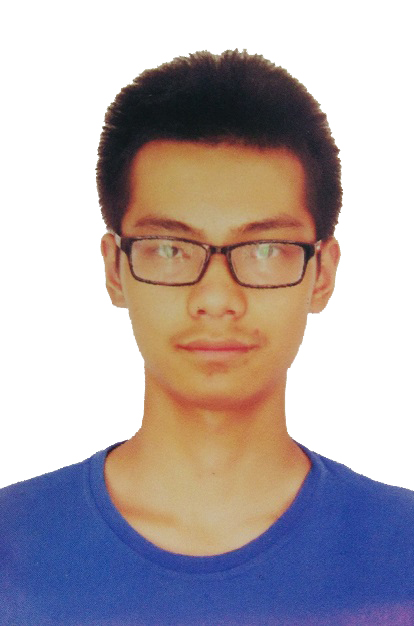
\includegraphics[width=0.88in]{images/profile.jpg}} & \faMale\
	\scshape{吴振宇}                                                         & {\faPython\ Python~}\progressbar{0.5}                                                                          \\
	                                                                      & \email{Wuzy01@qq.com}                                                  & {\faDraftingCompass\
	Julia~}\progressbar{0.6}                                                                                                                                                               \\
	                                                                      & \phone{+86~183~555~28308}                                              & {\faLinux\ Linux~}\progressbar{0.7}   \\
	                                                                      & \linkedin[zhenyu-wu]{https://www.linkedin.com/in/zhenyu-wu-5625971a7/} &
	{\faFile\ Tex~}\progressbar{0.8}                                                                                                                                                       \\
	                                                                      & \github[Freed-Wu]{https://www.github.com/Freed-Wu}                     & {\faVimeo\
	Vimscript~}\progressbar{0.9}                                                                                                                                                           \\
	                                                                      & \faQq\ 1295652958                                                      & {\faCuttlefish\ C~}\progressbar{0.65}
\end{tabu}
\normalsize

\section{\faGraduationCap\ 教育}%
\label{sec:zh_education}

\datedsubsection{\faUniversity\ \textbf{南京理工大学}}{2016年9月 $\sim$ 现在}%
\label{sub:zh_njust}

\faGraduationCap\ \emph{学士}\ \faBolt\ 电子信息工程

\section{\faUsers\ 经历}%
\label{sub:zh_experience}

\datedsubsection{\faCar\ 南京理工大学电动方程式汽车队}{2017年10月 $\sim$ 2019年4月}%
\label{sub:zh_fsae}

\role{\faBolt\ 电子电气部}{\faMicrochip\ 嵌入式开发}
参与设计整车数据采集系统。实现数据远程传输;优化数据监控系统。

\datedsubsection{\faSchool\ 学校}{2019年9月 $\sim$ 现在}%
\label{sub:zh_school}

\role{\faUsers\ 班级}{\faUserCheck\ 班长}

\section{\faCogs\ 技能}%
\label{sec:zh_skills}

\begin{itemize}
	\item 编程:\faVimeo\ Vimscript > \faFile\ Tex >
	      \faDraftingCompass\ Julia > \faCuttlefish\ C > \faPython\ Python
	\item 平台:\faLinux\ Linux
	\item 开发:\faMicrochip\ 嵌入式 > \faFile\ 用户界面设计 > \faGlobeAsia\ 互联网
\end{itemize}

\section{\faHeart\ 荣誉}%
\label{sec:zh_honors}

\datedline{\faEnvelopeOpenText\ 专利:
	\href{http://epub.sipo.gov.cn/}{CN109255866A}}{2019年1月}
\datedline{\faEnvelopeOpenText\ 专利:
	\href{http://epub.sipo.gov.cn/}{CN109301609A}}{2019年2月}
\datedline{\faThumbsUp\ 国家奖学金}{2018年11月}
\datedline{\faThumbsUp\ 特等奖学金}{2018年9月}
\datedline{\faThumbsUp\ 华为奖学金}{2019年9月}
\datedline{\faThumbsUp\ 三好学生}{2019年10月}
\datedline{\faThumbsUp\ 优秀团干}{2020年6月}
\datedline{\faRocket\ 江苏省电子设计竞赛二等奖}{2018年8月}
\datedline{\faRocket\ 美国大学生数学建模竞赛二等奖}{2018年1月}
\datedline{\faRocket\ 大学生高等数学竞赛一等奖}{2018年11月}

\section{\faInfo\ 其它}%
\label{sec:zh_miscellaneous}

\begin{itemize}
	\item\faBlog\ 个人博客: \url{https://Freed-Wu.github.io/}
	\item\faLanguage\ 语言: 英语(四六级), 普通话(普通话等级考试)
\end{itemize}

\end{document}
